\documentclass[a5paper,headsepline,titlepage,11pt,nnormalheadings,DIVcalc]{scrbook}
\usepackage[a5paper,backref]{hyperref}
\usepackage[papersize={148.5mm,215mm},twoside,bindingoffset=0.5cm,hmargin={2cm,2cm},
vmargin={2cm,2cm},footskip=1.1cm,driver=dvipdfm]{geometry}
%\usepackage{palatino}
\usepackage{graphicx}
\usepackage{wrapfig}
\usepackage[bahasa]{babel}
\usepackage{fancyhdr}
\usepackage{longtable}
\usepackage{hhline,multirow}
\usepackage{pst-node}

%\setlength{\voffset}{0.5in}
%\setlength{\oddsidemargin}{28pt}
%\setlength{\evensidemargin}{0pt}
\renewcommand{\footrulewidth}{0.5pt}
\lhead[\fancyplain{}{\thepage}]%
      {\fancyplain{}{~}}
\rhead[\fancyplain{}{~}]%
      {\fancyplain{}{\thepage}}
\pagestyle{fancy}
\lfoot[\emph{Doa 40 hari \namaalm}]{}
\rfoot[]{\emph{Lingkungan St Petrus Maguwo}}
\cfoot{}

\newcommand{\BU}[1]{\begin{itemize} \item[U:] #1 \end{itemize}}
\newcommand{\BI}[1]{\begin{itemize} \item[I:] #1 \end{itemize}}
\newcommand{\BP}[1]{\begin{itemize} \item[P:] #1 \end{itemize}}
\newcommand{\BPP}[1]{\begin{itemize} \item[Bpk:] #1 \end{itemize}}
\newcommand{\BPW}[1]{\begin{itemize} \item[Ibu:] #1 \end{itemize}}
\newcommand{\namaalm}{Ibu MG Ari Tri Wuryanti~}
\newcommand{\namaromo}{~}
\newcommand{\peringatan}{100 hari~}
\title{Ibadat/Doa untuk Arwah}
\author{}
\date{2010}
\hyphenation{a-kan}
\hyphenation{ba-gi-mu}
\hyphenation{ber-a-da}
\hyphenation{ber-du-a}
\hyphenation{be-ri-kan}
\hyphenation{ber-ka-ta}
\hyphenation{ber-nya-nyi}
\hyphenation{ber-sa-ma}

\hyphenation{dah-syat}
\hyphenation{DA-RAH-KU}
\hyphenation{da-tang}
\hyphenation{di-ka-ta-kan}
\hyphenation{di-pim-pin}
\hyphenation{di-se-rah-kan}
\hyphenation{di-tum-pah-kan}

\hyphenation{Eng-kau}
\hyphenation{ha-dap-an}
\hyphenation{han-tar-kan-lah}
\hyphenation{ha-rap-an}

\hyphenation{ja-lan}
\hyphenation{ja-ngan-lah}

\hyphenation{ka-nak}
\hyphenation{ka-re-na}
\hyphenation{kau-lim-pah-kan}
\hyphenation{Kau-cip-ta-kan}
\hyphenation{ke-bang-kit-an-Nya}
\hyphenation{ke-da-tang-an}
\hyphenation{ke-da-tang-an-Nya}
\hyphenation{ke-dua}
\hyphenation{ke-na-ik-kan-nya}
\hyphenation{ke-pa-daMu}
\hyphenation{ke-ra-him-an}
\hyphenation{ke-se-jah-te-ra-an-mu}
\hyphenation{ko-men-tar}

\hyphenation{la-ma-nya}
\hyphenation{lim-pah-kan}

\hyphenation{ma-nu-sia}
\hyphenation{me-nga-da-kan}
\hyphenation{me-ngan-dung-lah}
\hyphenation{me-ngu-kuh-kan}
\hyphenation{me-la-lui}
\hyphenation{me-lim-pah-kan}
\hyphenation{me-lu-hur-kan}
\hyphenation{me-me-cah-me-cah-kan}
\hyphenation{mem-per-sem-bah-kan}
\hyphenation{me-nan-da-ta-ngan-i}
\hyphenation{men-cin-tai}
\hyphenation{meng-a-lir-kan}
\hyphenation{me-nga-sihi}
\hyphenation{me-nge-lu-ar-kan}
\hyphenation{meng-u-cap-kan}
\hyphenation{meng-ung-kap-kan}
\hyphenation{me-num-buh-kan}
\hyphenation{me-nya-ta-kan}
\hyphenation{me-nye-la-mat-kan}
\hyphenation{me-nye-rah-kan}
\hyphenation{me-nye-rah-kanNya}
\hyphenation{me-ra-ya-kan}

\hyphenation{o-rang}
\hyphenation{o-rang-o-rang}

\hyphenation{pa-sang-kan-lah}
\hyphenation{pa-tut}
\hyphenation{pe-ne-ri-ma-an}
\hyphenation{pe-ngam-pun-an}
\hyphenation{Pe-ngan-ta-ra}
\hyphenation{peng-hi-bur-an}
\hyphenation{per-bu-at-an-nya}
\hyphenation{per-ka-ta-an}
\hyphenation{per-ka-win-an}
\hyphenation{per-ni-kah-an}
\hyphenation{per-se-ku-tu-an}
\hyphenation{per-sem-bah-an}
\hyphenation{rom-bong-an}

\hyphenation{se-la-ma}
\hyphenation{se-ka-li-an}
\hyphenation{se-pan-jang}
\hyphenation{se-ra-ya}
\hyphenation{Su-dar-yan-to}

\hyphenation{te-ta-pi}
\hyphenation{ta-ngan-Mu}
\hyphenation{Tu-han}
\hyphenation{tu-lang}
\hyphenation{tu-lang-tu-lang}

\hyphenation{u-mat-Mu}
\hyphenation{wa-kil}

\hyphenation{ba-gi-mu}
\hyphenation{di-se-rah-kan}
\hyphenation{me-la-lui}
\hyphenation{ka-nak}
\hyphenation{ka-re-na}
\hyphenation{ber-ka-ta}
\hyphenation{te-ta-pi}
\hyphenation{per-ka-win-an}
\hyphenation{pa-tut}
\hyphenation{me-lu-hur-kan}
\hyphenation{ber-nya-nyi}
\hyphenation{di-tum-pah-kan}
\hyphenation{pe-ngam-pun-an}
\hyphenation{ber-a-da}
\hyphenation{kau-lim-pah-kan}
\hyphenation{ke-bang-kit-an-Nya}
\hyphenation{per-ka-ta-an}
\hyphenation{pa-sang-kan-lah}
\hyphenation{DA-RAH-KU}
\hyphenation{ke-na-ik-kan-nya}
\hyphenation{per-sem-bah-an}
\hyphenation{per-se-ku-tu-an}


\renewcommand*\thesection{\arabic{section}.}
\setlength{\parindent}{0mm} 

\begin{document}
\thispagestyle{empty}
%\maketitle
%\newsavebox\IBox
%\sbox\IBox{\includegraphics[scale=0.4]{Saint-Peter-Apostle-e.eps}}

\psset{unit=1in}
\begin{pspicture}(4in,6.0in)
% set up the fonts we use
\DeclareFixedFont{\PT}{T1}{ppl}{b}{it}{0.4in}
\DeclareFixedFont{\PTsmall}{T1}{ppl}{b}{it}{0.3in}
\DeclareFixedFont{\PTsmallest}{T1}{ppl}{b}{it}{0.2in}
\DeclareFixedFont{\PTtext}{T1}{ppl}{b}{it}{11pt}
\DeclareFixedFont{\Logo}{T1}{pbk}{m}{n}{0.2in}
% place the front cover picture
%\rput[cb](2.3,2.5){\usebox\IBox}
% put the text on the front cover
\rput[cb](2.5,5.3){\PTsmall {Ibadat/Doa Arwah \peringatan untuk}}
\rput[cb](2.5,4.8){\PTsmall {\namaalm}}
\rput[cb](2.5,1.1){\PTsmall {9 Juni 2010}}
\rput[cb](2.5,0.6){\PTsmallest {Wilayah Yohanes de Britto}}
\rput[cb](2.5,0.3){\PTsmallest {Stasi Maguwo}}
\rput[cb](2.5,0.0){\PTsmallest {Paroki Marganingsih Kalasan }}

%\rput[cb](3,-1){\PTsmallest {\namagereja}} 

\end{pspicture}
%\tableofcontents 
\newpage
\thispagestyle{empty}
{~}
\newpage
\setlength{\parskip}{2mm}

\section*{RITUS PEMBUKA}
\subsection*{LAGU PEMBUKA}

\subsection*{SALAM PEMBUKAAN}
\BP{Atas nama Bapa Putera dan Roh Kudus} 
\BU{Amin}
\BP{Semoga damai sejahtera Tuhan kita Yesus Kristus, cinta kasih Allah Bapa dan persekutuan Roh Kudus, selalu beserta kita.}
\BU{Sekarang dan selama-lamanya}

\subsection*{PENGANTAR}
\BP{Bapak Ibu Saudara Saudari Anak-anak yang terkasih dalam Kristus, \peringatan yang lalu keluarga ini mengalami duka yang mendalam. Kalau ditanya mengapa berduka? Jawabanya adalah karena pada waktu itu \namaalm telah dipanggil Tuhan. Mungkin kita bisa ikut merasakan perasaan / suasana hati dari keluaraga yang ditinggalkan pada waktu itu. Sebagai ungkapan cinta keluarga ini terhadap almarhumah \namaalm kita semua diundang untuk bersama-sama mendukung dengan doa-doa supaya arwah dari \namaalm segera dapat ikut bangkit mulia bersama Kristus di dalam kerajaan surga.}

\emph{Hening sejenak \dots}
  
\subsection*{PERNYATAAN TOBAT}
\BP{Saudara-saudari yang seiman dalam Kristus, marilah kita membuat diri pantas berada di depan hadirat Allah, dengan membersihkan diri kita dari dosa dan kesalahan yang lalu, dengan bertobat dan mohon ampun kepada Allah kita.}

\BP{Selama kusembunyikan dosaku, batinku tertekan dan aku mengeluh sepanjang hari}
\BU{Berbahagialah orang, bila dosanya diampuni}
\BP{Aku mengakui dosaku di hadapanMu, Tuhan, dan kesalahanku tidak kusembunyikan}
\BU{Berbahagialah orang, bila dosanya diampuni}
\BP{Nasib orang berdosa sengsara belaka tetapi orang yang percaya kepada Tuhan dilimpahi kasih setia}
\BU{Berbahagialah orang, bila dosanya diampuni}
\BP{Semoga Allah yang mahakuasa mengasihani kita, 
mengampuni dosa kita dan mengantar kita ke dalam hidup 
yang kekal.}

\BU{Amin}

\subsection*{Doa Pembuka}
\BP{Marilah Berdoa 

Allah Bapa yang mahamurah, Engkau telah menyerahkan 
Yesus, Putra-Mu kepada kematian, semua ini harus terjadi 
untuk melepaskan kami dari segala kuasa kegelapan dan 
dosa. Ya Bapa, anugerahkanlah hidup kekal kepada 
saudara-saudari \namaalm yang telah menghadap 
kehadiratMu \peringatan yang lalu. Ya Bapa, ampunilah 
segala dosa dan kesalahannya dan bukalah pintu 
kehidupan kekal baginya. Terimalah saudara kami 
tercinta ini kedalam keluarga kudusMu di tahta surgawi. }

\BU{Amin} 
 
\section*{IBADAT SABDA}
\BP{Saudara-saudari terkasih marilah kita mempersiapkan hati 
dan budi untuk mendengarkan sabda Tuhan.} 

\subsection*{BACAAN PERTAMA}

\BP{Pembacaan dari Kitab Kebijaksanaan (3: 1-9) 

Tetapi jiwa orang benar ada di tangan Allah, dan siksaan tiada menimpa mereka.
Menurut pandangan orang bodoh mereka mati nampaknya, dan pulang mereka dianggap malapetaka,
dan kepergiannya dari kita dipandang sebagai kehancuran, namun mereka berada dalam ketenteraman.

Kalaupun mereka disiksa menurut pandangan manusia, namun harapan mereka penuh kebakaan.
Setelah disiksa sebentar mereka menerima anugerah yang besar, sebab Allah hanya menguji mereka, lalu mendapati mereka layak bagi diri-Nya.

Laksana emas dalam dapur api diperiksalah mereka oleh-Nya, lalu diterima bagaikan korban bakaran.
Maka pada waktu pembalasan mereka akan bercahaya, dan laksana bunga api berlari-larian di ladang jerami.
Mereka akan mengadili para bangsa dan memerintah sekalian rakyat, dan Tuhan berkenan memerintah mereka selama-lamanya.

Orang yang telah percaya pada Allah akan memahami kebenaran, dan yang setia dalam kasih akan tinggal pada-Nya. Sebab kasih setia dan belas kasihan menjadi bagian orang-orang pilihan-Nya.

Demikianlah sabda Tuhan }

\BU{Syukur kepada Allah} 

\subsection*{Antar Bacaan} 

\subsection*{Bacaan Injil} 

\BP{Tuhan sertamu} 
\BU{Dan sertamu juga} 
\BP{Inilah Injil Yesus Kristus menurut Lukas (7:11-17) 

Kemudian Yesus pergi ke suatu kota yang bernama Nain. Murid-murid-Nya pergi bersama-sama dengan Dia, dan juga orang banyak menyertai-Nya berbondong-bondong.

Setelah Ia dekat pintu gerbang kota, ada orang mati diusung ke luar, anak laki-laki, anak tunggal ibunya yang sudah janda, dan banyak orang dari kota itu menyertai janda itu.
Dan ketika Tuhan melihat janda itu, tergeraklah hati-Nya oleh belas kasihan, lalu Ia berkata kepadanya: "Jangan menangis!"
Sambil menghampiri usungan itu Ia menyentuhnya, dan sedang para pengusung berhenti, Ia berkata: "Hai anak muda, Aku berkata kepadamu, bangkitlah!"
Maka bangunlah orang itu dan duduk dan mulai berkata-kata, dan Yesus menyerahkannya kepada ibunya.

Semua orang itu ketakutan dan mereka memuliakan Allah, sambil berkata: "Seorang nabi besar telah muncul di tengah-tengah kita," dan "Allah telah melawat umat-Nya."
Maka tersiarlah kabar tentang Yesus di seluruh Yudea dan di seluruh daerah sekitarnya.

Demikianlah Injil Tuhan} 

\BU{Terpujilah Kristus}

\subsection*{HOMILI}

Gagasan homili
\begin{itemize}
\item Yesus tergerak menolong. Ibu gembira anaknya kembali segar bugar
\item Keprihatinan Yesus terus berlanjut sampai sekarang bagi yang membutuhkan
\item Kesedihan masih terasa
\item Berkat wafatNya Yesus memberikan kebahagiaan abadi kepada \namaalm
\item Jika orang benar di tangan Allah, siksaan tiada menimpa mereka
\item Tetap setia kepada Allah berharap dapat merasakan belas kasih Allah.
\end{itemize}

Marilah kita lanjutkan dengan doa umat

\section*{DOA}

\subsection*{DOA UMAT}

\BP{Allah Bapa kami yang maha kasih dan penyayang, kami menghadap hadiratmu untuk menyampaikan ungkapan hati dan permohonan kami. Kami percaya Engkau akan selalu berkenan menyertai kami, mendengarkan kami dan memberikan yang terbaik bagi kami. Kami memuji dan memuliakan nama-Mu melalui doa-doa ini:}

\BP{Ya Tuhan Yesus Kristus penyelamat dunia kami mempercayakan kepadamu arwah \namaalm, berkenanlah engkau menerimanya dalam sukacita kerajaan-Mu

Kami mohon}

\BU{Kabulkanlah doa kami ya Tuhan}

\BP{Ya Allah, kami mohon kemurahaanmu bagi \namaalm , janganlah kau ingat-ingat lagi dosa-dosanya, tetapi limpahkanlah kerahiman-Mu kepadanya. Semoga Ia disambut dan dipersatukan bersama para malaikat dan orang kudus di surga.

Kami mohon}

\BU{Kabulkanlah doa kami ya Tuhan}

\BP{Bagi keluarga yang ditinggalkan, ya Bapa tolonglah mereka semua supaya saling mendukung , saling memberi kekuatan dan penghiburan. Semoga kenangan akan masa hidup \namaalm akan tersimpan dalam hati mereka, dan meneguhhkan kepercayaan mereka akan bimbingan-Mu 

Kami mohon}

\BU{Kabulkanlah Doa kami ya Tuhan} 

\BP{Ya Bapa Keluarga ini telah menyerahkan seluruh hidupnya kedalam penyelenggaraan-Mu, maka sudilah mendampingi mereka supaya sanggup menghadapi liku-liku hidup ini , lebih-lebih saat ini dikala keluarga ini ditinggalkan oleh ibu yang mereka cintai.

Kami mohon}

\BU{Kabulkanlah doa kami ya Tuhan}

\BP{Bagi kita semua yang berhimpun disini beserta keluarganya, ya Bapa jadikanlah kami alat-Mu dalam menciptakan kerukunan dan penghiburan dan pembawa damai. Jauhkanlah kami semua dari kemalangan.

Kami mohon}

\BU{Kabulkanlah doa kami ya Tuhan}

\BP{Demikianlah ya Bapa, doa-doa yang kami panjatkan. Engkau mengetahui keinginan keinginan dan kesulitan kami. Kami percaya akan penyelenggaraan-Mu dan bersama Roh Kudus, kami senantiasa belajar utuk memahami apa yang sebenarnya Engkau kehendaki atas diri kami . Kami menyampaikan doa-doa kami ini dengan perantaraan Putera-Mu terkasih, Tuhan kami Yesus Kristus, yang hidup dan berkuasa kini dan sepanjang masa. Amin}


\subsection*{DOA BAPA KAMI}
Marilah kita satukan doa-doa permohonan kita dengan doa yang diajarkan Yesus sendiri 
Bapa kami yang ada di surga \dots .( didoakan bersama sama )

\subsection*{ROSARIO}
Bapak Ibu Saudara Saudari, Ibu Maria telah memberikan teladan bagi kita. Ia telah setia mendampingi Puteranya Tuhan Yesus Kristus sampai wafatnya di kayu salib. Marilah kita mohon lewat perantaraan Bunda Maria supaya arwah \namaalm lancar dalam menghadap Bapa dengan doa Rosario.

Aku percaya

Bapa kami \dots

Kemuliaan kepada Bapa \dots

Terpujilah \dots

Salam Putri Allah Bapa. Salam Maria \dots

Salam Bunda Allah Putera. Salam Maria \dots 

Salam Mempelai Allah Roh Kudus. Salam Maria \dots

Kemuliaan \dots

Terpujilah \dots

Ya Bapa terimah arwah \namaalm dalam kemuliaan kerajaan-Mu.

\section*{RITUS PENUTUP}

\subsection*{DOA PENUTUP}
\BP{Marilah berdoa :
 
Allah Bapa kami yang mahapengasih dan penyayang, 
semoga kebangkitan putraMu juga menjadi kebangkitan 
saudara kami \namaalm  Bapa semoga Engkau senantiasa 
membangkitkan semangat kami untuk terus menerus hidup 
seturut nasihat InjilMu. Bapa, semoga doa-doa yang kami 
panjatkan kehadiratMu mampu mengantar saudara-saudari 
kami yang sudah meninggal untuk memasuki kerajaanMu 
yang abadi di surga. }
\BU{Amin}

\subsection*{BERKAT}
\BP{Tuhan beserta kita}
\BU{Sekarang dan selama-lamanya}
\BP{Semoga kita semua, keluarga kita dan karya kita selalu di bimbing dan diberkati oleh Bapa dan Putera dan Roh Kudus.}

\BU{Amin}

\BP{Saudara sekalian ibadat kita sudah selesai marilah kita mundur dalam damai Tuhan}
\BU{Syukur kepada Allah.}

\subsection*{LAGU PENUTUP}

\end{document}